%Incluímos el archivo contenedor de paquetes y definiciones del documento
\documentclass[11pt,a4paper]{article}
\usepackage[utf8]{inputenc}
\usepackage[spanish]{babel}
\usepackage{amsmath}
\usepackage{amsfonts}
\usepackage{amssymb}
\usepackage{graphicx}
\usepackage{hyperref}
\usepackage[left=3cm,right=3cm,top=3cm,bottom=3cm]{geometry}
\usepackage{float}
\renewcommand{\P}{\ensuremath{\textup{\textbf{P}}}}
\newcommand{\E}{\ensuremath{\textup{\textbf{E}}}}

\title{\huge{\textbf{Análisis asintótico de algoritmos}}}
\author{\large{\textbf{Sergio Revilla Velasco}}}
\date{}

\begin{document}
\maketitle

%Resumen del documento (Abstract)

\begin{abstract}
%\noindent
El objetivo de esta práctica es estudiar la complejidad asintótica de los algoritmos de ordenación más comunes (selección (selection-sort), inserción (insertion-sort), burbuja (bubble-sort), ordenación rápida (quick-sort) y ordenación por mezcla (merge-sort)) por medio de un programa escrito en \textbf{C++}.
\end{abstract}


%Muestra el índice generado por las secciones y subsecciones
\tableofcontents{}

%\setlength{\parindent}{0pt}

%Incluimos las secciones del artículo
\section{Instrucciones de compilación y dependencias}
\begin{enumerate}
	\item \textbf{Dependencias:}
		\begin{itemize}
			\item \textbf{Windows:}  MinGW  \url{http://www.mingw.org}
			\item \textbf{Linux:} GCC Compiler Collection  \url{http://gcc.gnu.org}
			\item \textbf{Mac Os X:} Xcode Tools con utilidades de línea de comando instaladas  							\url{https://developer.apple.com/xcode/}
			\item \textbf{GnuPlot:}  usado para generar las gr\'aficas desde archivos de texto 								\url{http://www.gnuplot.info}
		\end{itemize}
	\item \textbf{Instrucciones de compilaci\'on:}
			\begin{itemize}
			\item Compilar el archivo \textbf{"main.cpp"} contenido en la carpeta \textbf{"src"}
			\item Ejecutar desde la consola el comando \textbf{"gnuplot script.gnuplot"} desde el 					mismo directorio donde se generaron los archivos de datos.
			\item El script generar\'a archivos \emph{png} con las gr\'aficas.
			\end{itemize}
\end{enumerate}
\section{Proleg\'omenos}
Todos los algoritmos analizados en este trabajo parten de unas precondiciones y postcondiciones comunes a toda especificación de algoritmo de ordenación, esto es, partiendo de un array de números enteros positivos de tamaño $n > 0$, construimos un nuevo array con los elementos ordenados.  La especificación formal puede expresarse como:
\begin{itemize}
\item \textbf{Precondición:}\\
$P \equiv \{lon(V) = n > 0 \wedge V[n] \geq 0\}$ (Vector no vacío de enteros positivos)
\item \textbf{Definición:}\\$ordena(int \:\: \&V[],\: int \:n)$ (Devuelve el vector ordenado por referencia)
\item \textbf{Postcondición:}\\
$Q \equiv \{\forall{i} : 0 \leq i < n - 1: V[i] \leq V[i + 1]\}$
\end{itemize}
O expresado de otra manera:\cite{CORMEN} 
\begin{itemize}
\item \textbf{Entrada:} una secuencia de $n$ enteros positivos $(a_{1}, a_{2}, a_{3}, \:  \ldots\: , a_{n})$
\item \textbf{Salida:} una permutación (reordenación) de la secuencia de entrada tal que $(a_{1} \leq a_{2}  \leq a_{3},\:  \ldots\:  , \leq  a_{n})$
\end{itemize}

Cada método de ordenación se expresa como un algoritmo: un procedimiento de cálculo bien definido que toma algún valor o conjunto de valores como entrada y produce un cierto valor o conjunto de valores como salida.\cite{CORMEN} 

\section{Método de obtención de tiempos y gráficas}
	\begin{enumerate}
		\item El programa preguntará por el tamaño del problema (la longitud del array)
		\item También podemos elegir el mayor entero a generar (un entero puede tener un valor 				máximo de $2147483647$ )
		\item El programa preguntará por el salto \emph{(gap)} entre iteraciones.  Cuanto menor 					sea el tamaño de la iteración, más ajustada será la gráfica.  Para asegurarnos que 					recorremos hasta el último elemento del array el salto debe ser múltiplo de $5$.
		\item En primera instancia se genera un array con números aleatorios que sirve como base 					para las ordenaciones.  De esta manera las copias del array original se hacen del 					tamaño que corresponde a la iteración.  Así, si el tamaño del array a ordenar en cada iteración es de $n$ 					elementos, el programa copia el array en intervalos de $gap$ elementos hasta alcanzar el tamaño máximo del problema $(n)$.
		\item El programa genera un archivo con los datos separados por un salto de línea.  Cada 					línea contiene el tamaño del problema y el tiempo empleado para la ordenación expresado 			en segundos.
		\item Con los archivo de datos, puede ejecutarse el script de órdenes con la sintaxis de 				\textbf{gnuplot} para crear los arhivos de imagen con las gráficas de las métricas 					generadas.
	\end{enumerate}


\section{Análisis de resultados}
\begin{itemize}
\item Tamaño del problema: $100000$\footnote{Todos los resultados han sido generados en un ordenador Apple Imac, Mac Os X 10.8.2, Procesador Intel Core i5 a 2,5Ghz (4 núcleos), 4 Gb de RAM a 1333 Mhz DDR3.}
\item Máximo entero generado: $125000$
\item Salto entre iteraciones: $100$
\end{itemize}
\newpage
%Gráfica de ordenación por inserción
\subsection{Ordenación por inserción \cite{CORMEN}}
Su complejidad es de $O(n^2)$. Un buen algoritmo de ordenación para un número pequeño elementos. Funciona de la manera análoga a la que se ordenaría un mazo de cartas:
\begin{enumerate}
	\item Empezamos con la mano izquierda vacía y las cartas boca abajo sobre la mesa.
	\item A continuación, cogemos una carta de la mesa, y la insertamos en la posición correcta 			en la mano izquierda.
	\item Para encontrar la posición correcta en la que insertar la carta, se compara con cada 			una de las cartas que ya tenemos en la mano izquierda, recorriendo de derecha a 					izquierda.
\item En todo momento, las cartas sujetas con la mano izquierda se ordenan, permaneciendo las 			cartas originales sin ordenar encima de la pila en la mesa.
\end{enumerate}

	\begin{figure}[H]
  		\centering
   		 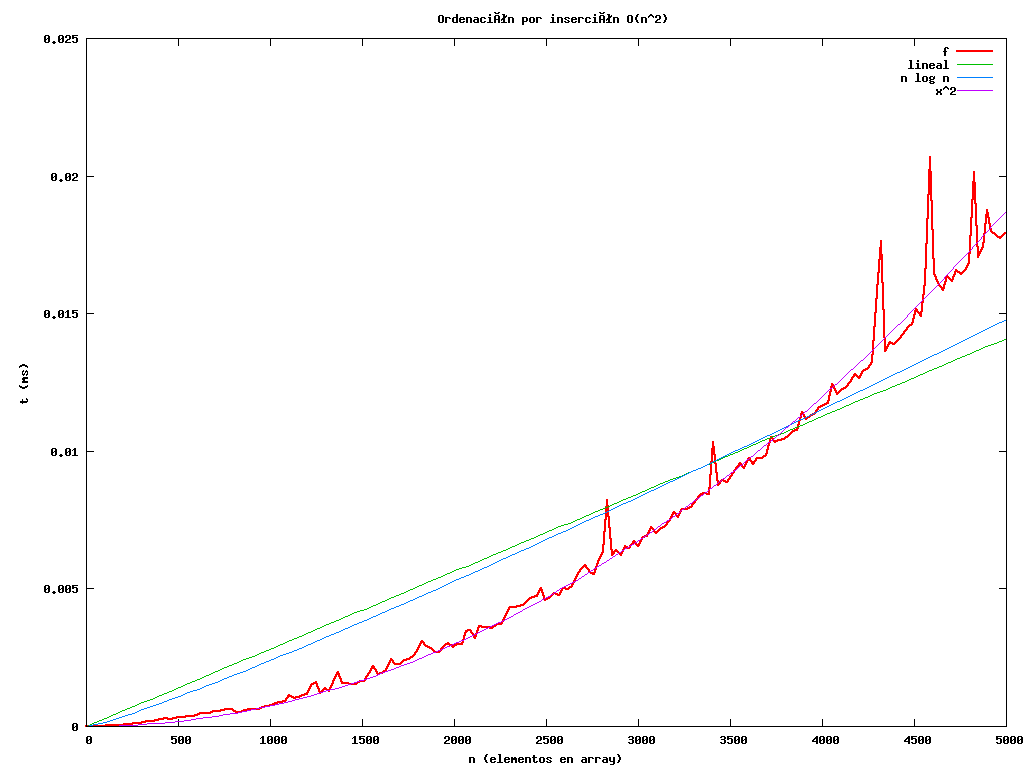
\includegraphics[width=1.0\textwidth]{insertion-sort.png}
  		\caption{Ordenación por inserción}
 			 \label{fig:insertion}
		\end{figure}

\newpage
%Gráfica de ordenación por selección
\subsection{Ordenación por selecci\'on}
Es un algoritmo de ordenación por comparación. Su complejidad es de $O(n^2)$. Resulta ineficiente en tamaños de problema grandes, y suele funcionar peor que la ordenación por inserción. Se caracteriza por su sencillez, y también tiene ventajas de rendimiento sobre algoritmos más complicados en determinadas situaciones, sobre todo cuando la memoria auxiliar es limitada.\\
El algoritmo divide la lista de entrada en dos partes: la lista secundaria de los elementos que ya están ordenados, dispuestos de izquierda a derecha, y la lista secundaria de los elementos restantes a ser ordenados, ocupando el resto de la lista. Inicialmente, la sublista ordenada está vacía y la sublista sin ordenar es la lista original menos los elementos ordenados. El algoritmo continúa encontrando siempre el elemento inmediatamente superior (según orden de clasificación) y lo cambia con el último elemento del array.

	\begin{figure}[H]
	  \centering
	    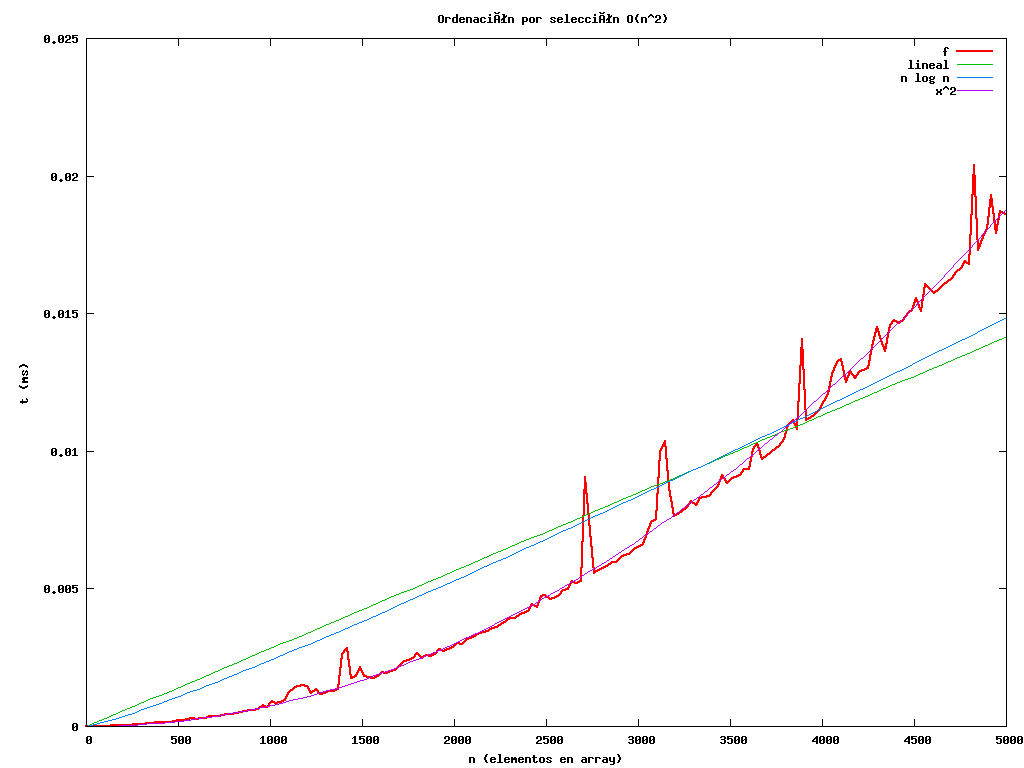
\includegraphics[width=1.0\textwidth]{selection-sort.png}
	  \caption{Ordenación por selección}
	  \label{fig:selection}
	\end{figure}

\newpage
%Gráfica de ordenación por burbuja
\subsection{Ordenación por burbuja}
Es un algoritmo por comparación.  Recorremos los elementos del array de derecha a izquierda, comparando cada elemento con el siguiente e intercambiándolos en caso de estar desordenados.
\subsubsection{Rendimiento}
Para ordenar un vector de $n$ elementos, el algoritmo siempre realiza el mismo número de comparaciones:
\[n\]
	\begin{figure}[H]
	  \centering
	    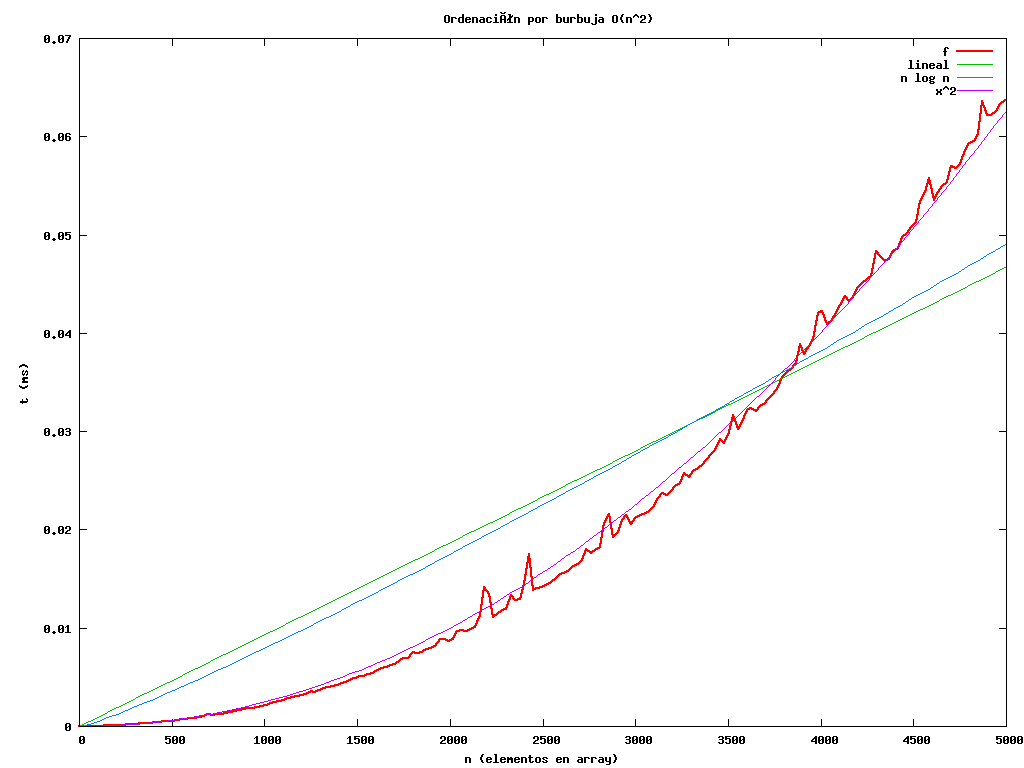
\includegraphics[width=1.0\textwidth]{bubble-sort.png}
	  \caption{Ordenación por burbuja}
	  \label{fig:bubble}
	\end{figure}

%Gráfica de ordenación rápida
\subsection{Ordenación r\'apida}

	\begin{figure}[H]
  		\centering
   	 	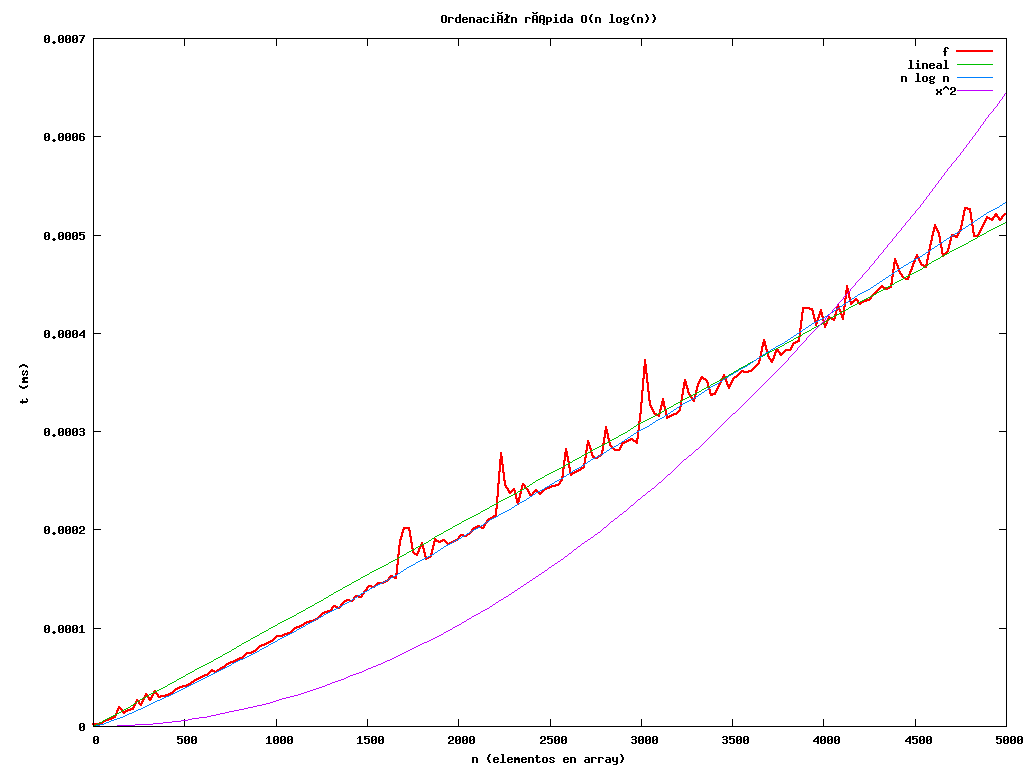
\includegraphics[width=1.0\textwidth]{quick-sort.png}
  		\caption{Ordenación rápida}
  		\label{fig:quick}
	\end{figure}
	
\subsection{Ordenación por mezcla}

	\begin{figure}[H]
  		\centering
   	 	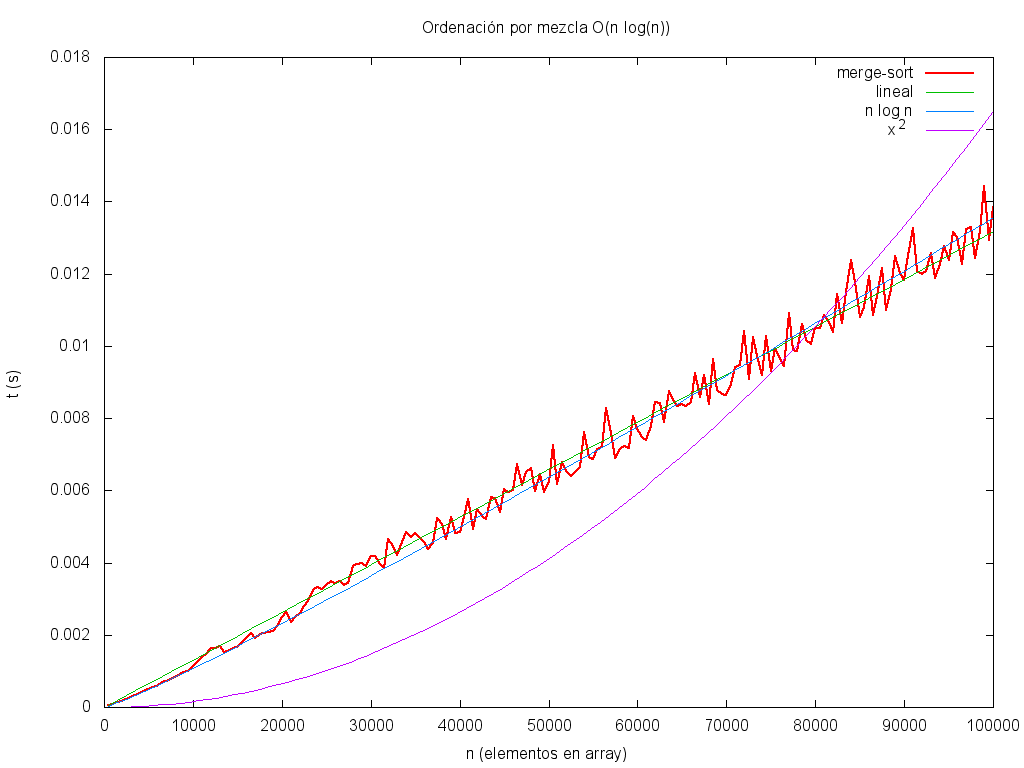
\includegraphics[width=1.0\textwidth]{merge-sort.png}
  		\caption{Ordenación por mezcla}
  		\label{fig:merge}
	\end{figure}

\section{Análisis de resultados}
Todos los resultados han sido generados en un ordenador Apple MacBook Pro, Mac Os X 10.8.2, Procesador Intel Core i5 a 2,4Ghz (4 núcleos), 4 Gb de RAM a 1333 Mhz DDR3.
\begin{itemize}
\item Tamaño del problema: $50000$
\item Máximo entero generado: $32767$
\item Salto entre iteraciones: $100$
\end{itemize}

%Gráfica de ordenación por inserción
\subsection{Ordenación por inserción \cite{CORMEN}}
Su complejidad es de $O(n^2)$. Un buen algoritmo de ordenación para un número pequeño elementos. Funciona de la manera análoga a la que se ordenaría un mazo de cartas:
\begin{enumerate}
	\item Empezamos con la mano izquierda vacía y las cartas boca abajo sobre la mesa.
	\item A continuación, cogemos una carta de la mesa, y la insertamos en la posición correcta 			en la mano izquierda.
	\item Para encontrar la posición correcta en la que insertar la carta, se compara con cada 			una de las cartas que ya tenemos en la mano izquierda, recorriendo de derecha a 					izquierda.
\item En todo momento, las cartas sujetas con la mano izquierda se ordenan, permaneciendo las 			cartas originales sin ordenar encima de la pila en la mesa.
\end{enumerate}

	\begin{figure}[H]
  		\centering
   		 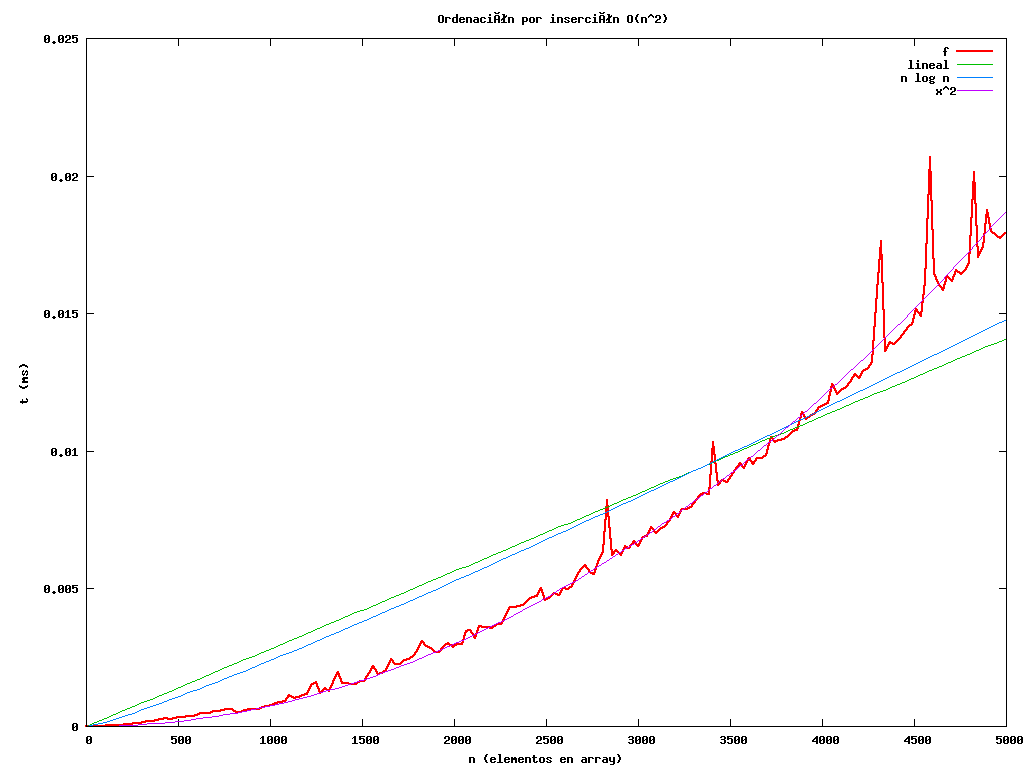
\includegraphics[width=1.0\textwidth]{insertion-sort.png}
  		\caption{Ordenación por inserción}
 			 \label{fig:insertion}
		\end{figure}

%Gráfica de ordenación por selección
\subsection{Ordenación por selecci\'on}
Es un algoritmo de ordenación por comparación. Su complejidad es de $O(n^2)$. Resulta ineficiente en tamaños de problema grandes, y suele funcionar peor que la ordenación por inserción. Se caracteriza por su sencillez, y también tiene ventajas de rendimiento sobre algoritmos más complicados en determinadas situaciones, sobre todo cuando la memoria auxiliar es limitada.
El algoritmo divide la lista de entrada en dos partes: la lista secundaria de los elementos que ya están ordenados, dispuestos de izquierda a derecha, y la lista secundaria de los elementos restantes a ser ordenados, ocupando el resto de la lista. Inicialmente, la sublista ordenada está vacía y la sublista sin ordenar es la lista original menos los elementos ordenados. El algoritmo continúa encontrando siempre el elemento inmediatamente superior (según orden de clasificación) y lo cambia con el último elemento del array.

	\begin{figure}[H]
	  \centering
	    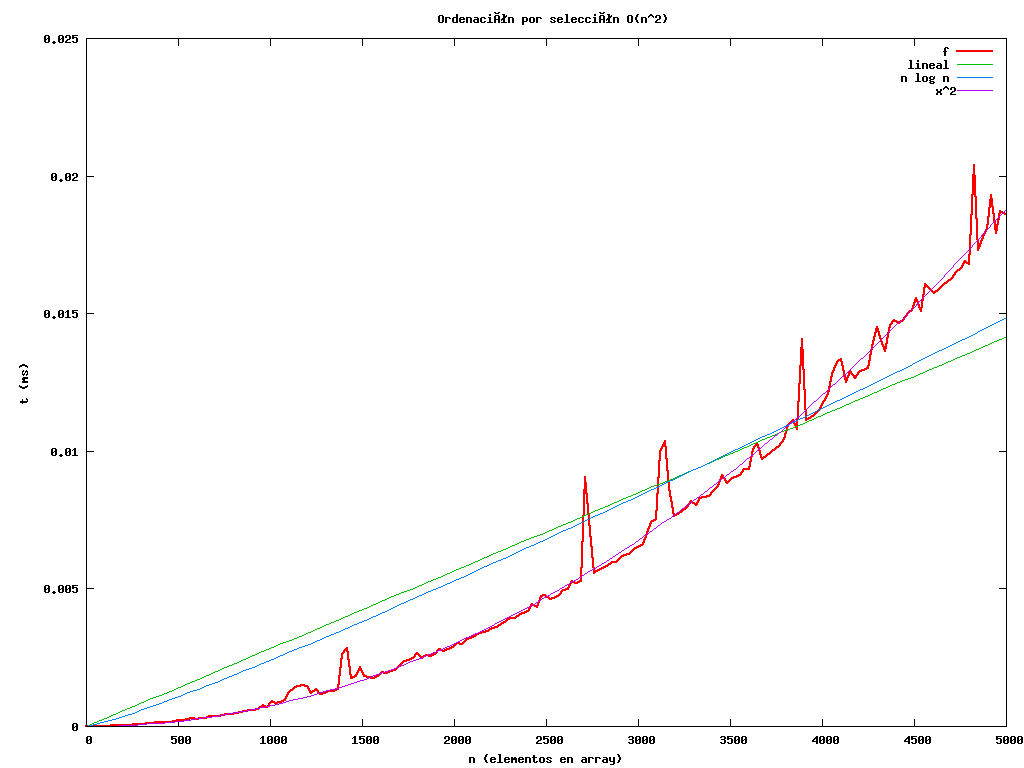
\includegraphics[width=1.0\textwidth]{selection-sort.png}
	  \caption{Ordenación por selección}
	  \label{fig:selection}
	\end{figure}

%Gráfica de ordenación por burbuja
\subsection{Ordenación por burbuja}
Es un algoritmo por comparación.  Recorremos los elementos del array de derecha a izquierda, comparando cada elemento con el siguiente e intercambiándolos en caso de estar desordenados.
\subsubsection{Rendimiento}
Para ordenar un vector de $n$ elementos, el algoritmo siempre realiza el mismo número de comparaciones:
\[n\]
	\begin{figure}[H]
	  \centering
	    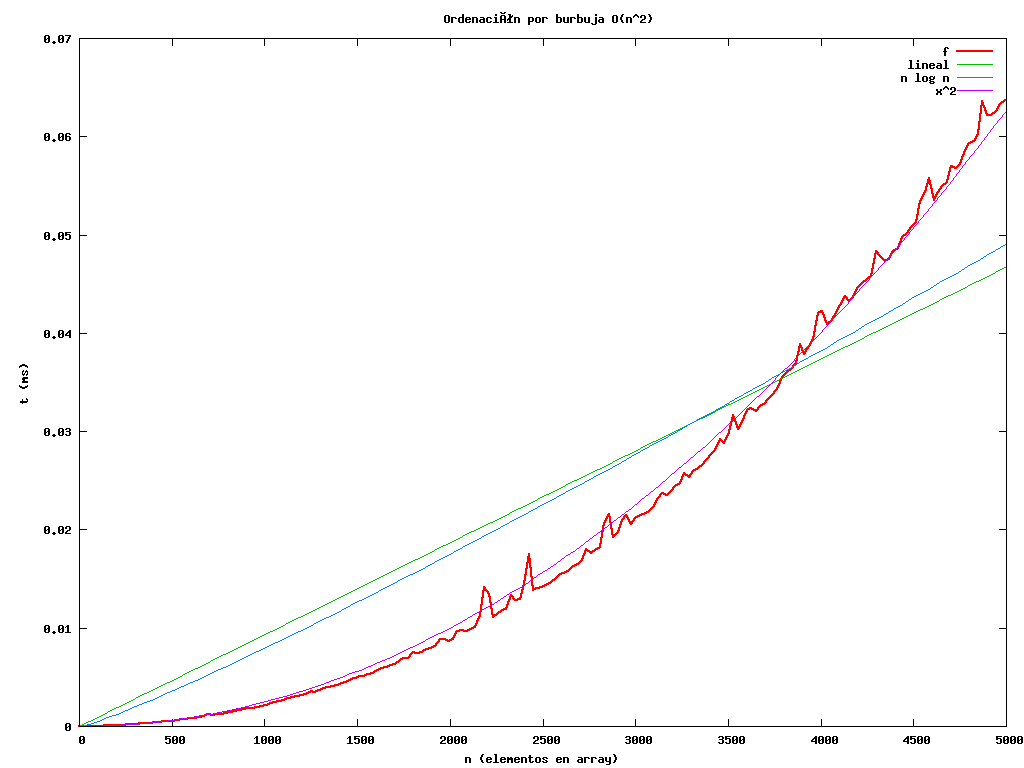
\includegraphics[width=1.0\textwidth]{bubble-sort.png}
	  \caption{Ordenación por burbuja}
	  \label{fig:bubble}
	\end{figure}

%Gráfica de ordenación rápida
\subsection{Ordenación r\'apida}

	\begin{figure}[H]
  		\centering
   	 	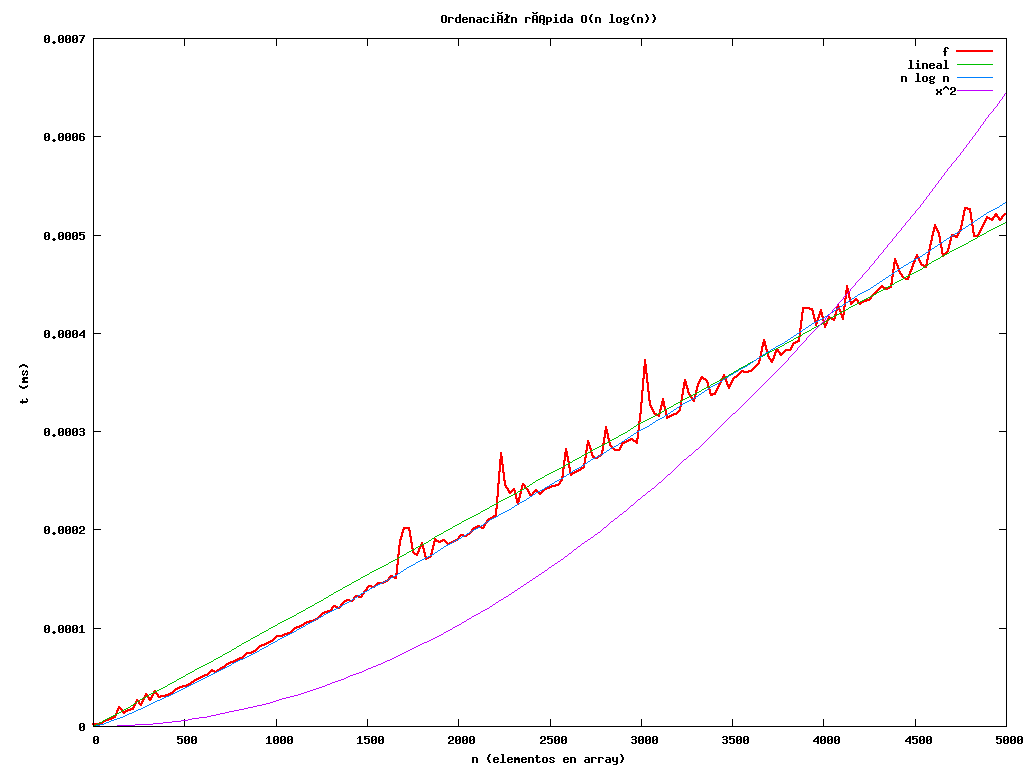
\includegraphics[width=1.0\textwidth]{quick-sort.png}
  		\caption{Ordenación rápida}
  		\label{fig:quick}
	\end{figure}


\section{Comentarios adicionales}

\begin{thebibliography}{10}

\bibitem{CORMEN} Cormen, Thomas H. and Leiserson, Charles E. and Rivest, Ronald L. and Stein, Clifford. \textit{Introduction to Algorithms, Third Edition}, MIT Press.  

\bibitem{EDA} Méndez, Gonzalo et al. \textit{Estucturas de datos y algoritmos}, UCM 2011 (Apuntes de clase).
\end{thebibliography}


\end{document}
